\documentclass[10pt,a4paper,twoside]{article}
\usepackage[utf8]{inputenc}
\usepackage[francais]{babel}
\usepackage[T1]{fontenc}
\usepackage[bitstream-charter]{mathdesign}
\usepackage[T1]{fontenc}
\usepackage{graphicx}
\usepackage{blindtext}
\usepackage{lipsum}
\usepackage[left=2cm,right=2cm,top=2cm,bottom=2cm]{geometry}
\author{Ludovic}
\title{\LaTeX \& Python pour de belles figures}
\begin{document}
\maketitle

\blindmathpaper

%\begin{figure}[htb]
\centerline{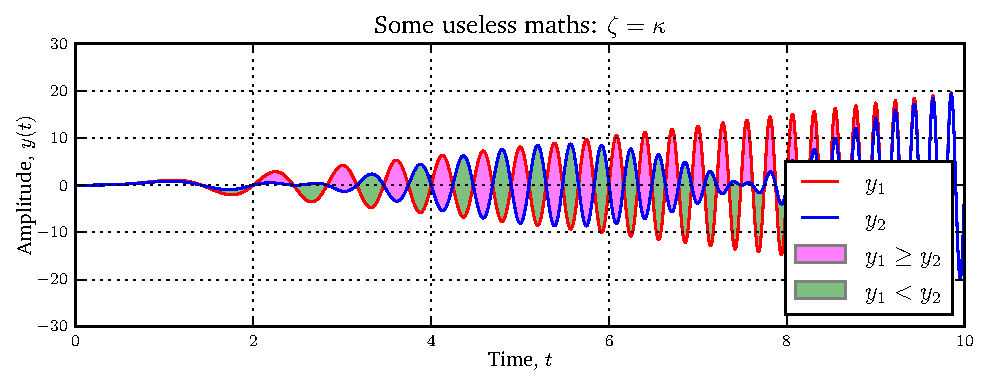
\includegraphics{fig}}
%\caption{ {\lipsum[2]} }
%\end{figure}

\blindmathpaper

\end{document}